% Template GRASS newsletter - Article
% Language: Latex
%

% Head
\graphicspath{{./images/}}

\title{Manipulations spatiales}
\subtitle{}
\author{}

\maketitle

La carte actuelle devrait \^etre comme ceci (plus ou moins):Fig.~\ref{fig:grass008}

%\setkeys{Gin}{width=1\textwidth}
\begin{figure}[htbp]
   \centering
   %name of your graphic, without the path AND in PNG (screnshots etc)/PDF (drawings) format:
   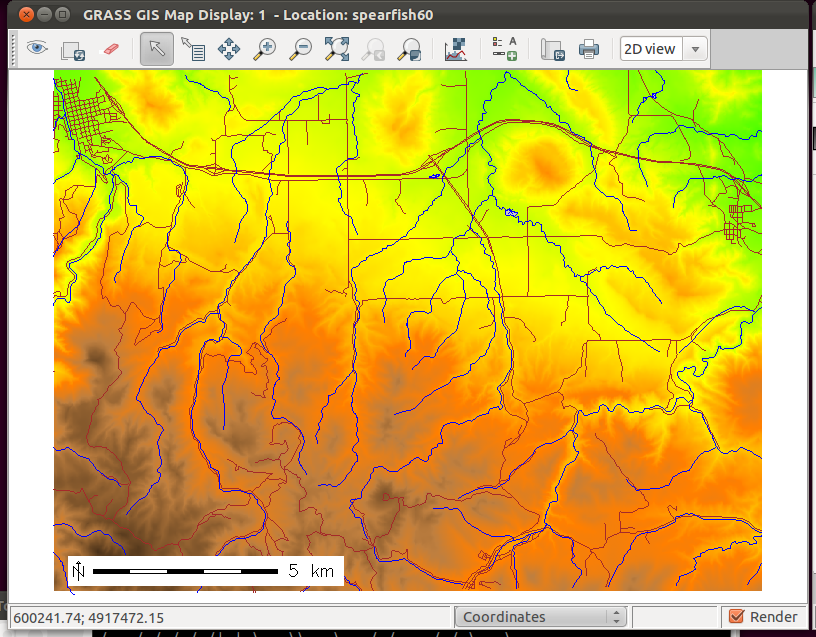
\includegraphics[scale=0.35]{grass008.png}
   %caption of the figure
   \caption{carte de travail pour cette section}
   %label of the figure, which has to correspond to \ref{}:
   \label{fig:grass008}
\end{figure}

\section{MANIPULATIONS DE DEM}
Affichage du DEM en des\'electionnant les vecteurs roads et streams Fig.~\ref{fig:grass009}

%\setkeys{Gin}{width=1\textwidth}
\begin{figure}[htbp]
   \centering
   %name of your graphic, without the path AND in PNG (screnshots etc)/PDF (drawings) format:
   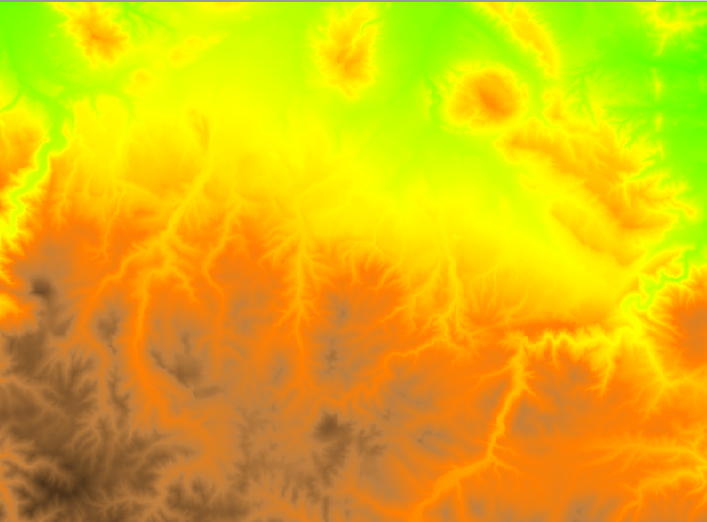
\includegraphics[scale=0.35]{grass009.png}
   %caption of the figure
   \caption{Affichage du DEM}
   %label of the figure, which has to correspond to \ref{}:
   \label{fig:grass009}
\end{figure}

\subsection{Calcul de pente et d'aspect}
Dans GRASS Tools, dans Region, changez la r\'esolution et mettez la \`a 10m x 10m. Puis recherchez r.slope, utilisez le avec la couche ''elevation.10m'', la carte d'aspect a \'et\'e pr\'epar\'ee \`a la fin de la section pr\'ec\'edente Fig.~\ref{fig:grass010}

%\setkeys{Gin}{width=1\textwidth}
\begin{figure}[htbp]
   \centering
   %name of your graphic, without the path AND in PNG (screnshots etc)/PDF (drawings) format:
   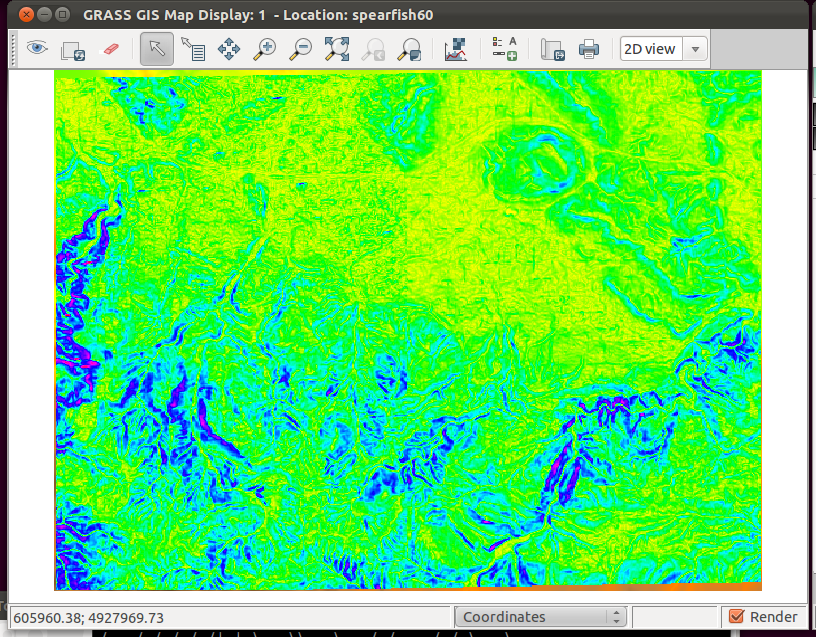
\includegraphics[scale=0.35]{grass010.png}
   %caption of the figure
   \caption{Pente}
   %label of the figure, which has to correspond to \ref{}:
   \label{fig:grass010}
\end{figure}

Calcul de carte de relief ombrag\'e (cherchez r.relief ou ''shaded'' ).
La carte de relief ombrag\'e devrait \^etre comme ceci quand la carte "elevation.10m" est superimpos\'ee dessus avec une opacit\'e de 0.75: Fig.~\ref{fig:grass011}

%\setkeys{Gin}{width=1\textwidth}
\begin{figure}[htbp]
   \centering
   %name of your graphic, without the path AND in PNG (screnshots etc)/PDF (drawings) format:
   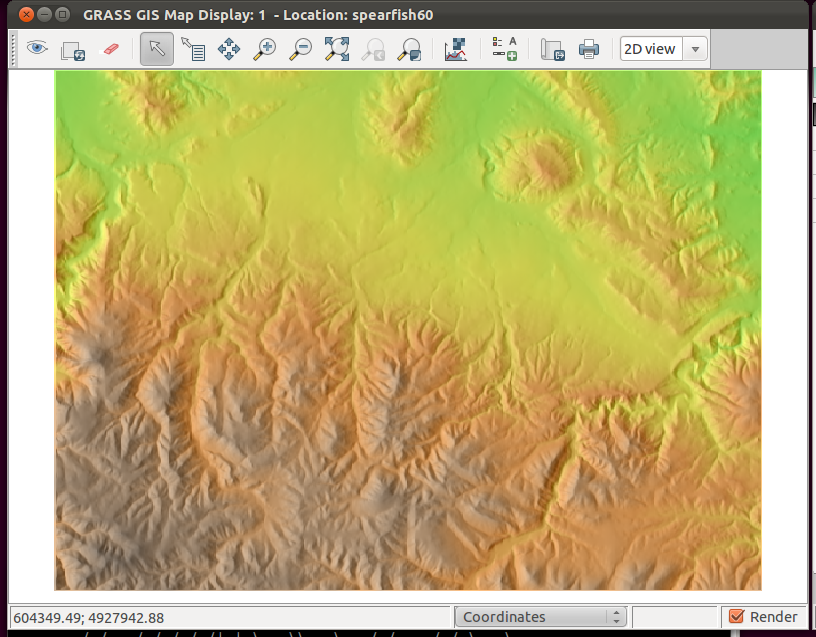
\includegraphics[scale=0.35]{grass011.png}
   %caption of the figure
   \caption{Relief Ombrag\'e}
   %label of the figure, which has to correspond to \ref{}:
   \label{fig:grass011}
\end{figure}

\subsection{Programme d'analyse de basin versant}
Trouvez r.watershed.\\
Remplissezs les param\`etres d'entr\'e de la carte d'altitude avec ''elevation.10m''. La taille minimum de l'ext\'erieur d'un bassin versant doit \^etre de 5000 pixels. Remplissez les param\`etres de sortie pour toutes les cartes disponibles (i.e. ''\_cells\_nbr'', ''\_drain\_dir'', ''\_drain\_dir'', ''\_basins'', ''\_streams'', ''\_half\_basins'', ''\_visual'', ''\_LS'', ''\_S'').

Voici ce que doit dire l' ex\'ecution du module:

SECTION 1a (of 6): Initiating Memory.

SECTION 1b (of 6): Determining Offmap Flow.

SECTION 2: A * Search. 

SECTION 3: Accumulating Surface Flow.

SECTION 4: Length Slope determination.

SECTION 5: Watershed determination.

SECTION 6: Closing Maps.

La carte r\'esultante ''\_basins'' devrait ressembler \`a cel\`a:Fig.~\ref{fig:grass012}

%\setkeys{Gin}{width=1\textwidth}
\begin{figure}[htbp]
   \centering
   %name of your graphic, without the path AND in PNG (screnshots etc)/PDF (drawings) format:
   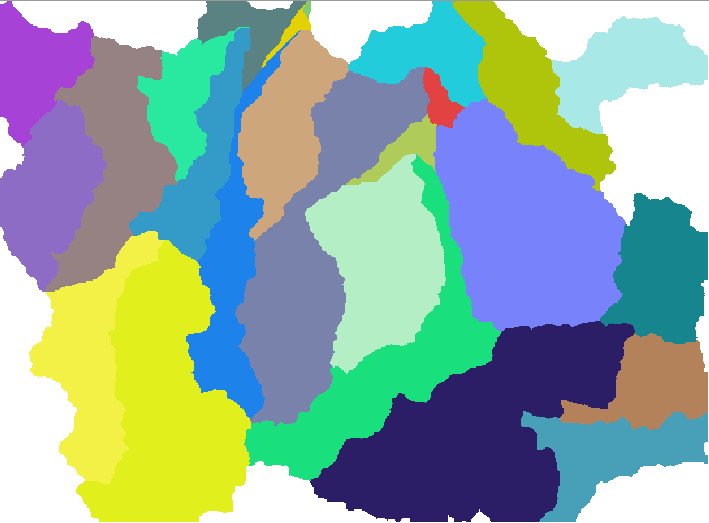
\includegraphics[scale=0.35]{grass012.png}
   %caption of the figure
   \caption{Carte de basins versants}
   %label of the figure, which has to correspond to \ref{}:
   \label{fig:grass012}
\end{figure}


La carte r\'esultante ''\_streams'' devrait ressembler \`a cel\`a: Fig.~\ref{fig:grass013} comparez-l\`a avec la carte vectorielle ''streams''.

%\setkeys{Gin}{width=1\textwidth}
\begin{figure}[htbp]
   \centering
   %name of your graphic, without the path AND in PNG (screnshots etc)/PDF (drawings) format:
   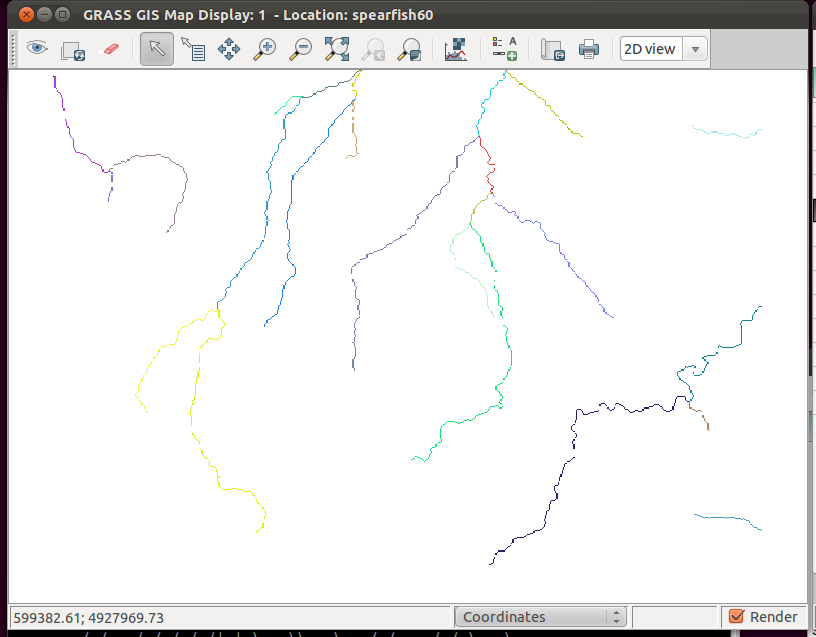
\includegraphics[scale=0.35]{grass013.png}
   %caption of the figure
   \caption{Carte de r\'eseau hydrologique}
   %label of the figure, which has to correspond to \ref{}:
   \label{fig:grass013}
\end{figure}

Relancez avec des valuers diff\'erentes au lieu de 5000 pixels, i.e. 2000 et 10000.
Comparez en vectorisant les r\'eseaux hydrologiques g\'en\'er\'es. La vectorisation se fait en cherchant ''v.out.'' dans GRASS Tools.

\subsection{Identification de site de station de suivit de la Pollution d'un ruisseau}
En consid\'erant qu'une usine de transformation/traitement de bois fasse une demande de permis pour mettre en place une nouvelle usine dans le basin versant. La localisation est distante du r\'eseau hydrologique majeur cartographi\'e (598713.35(E) 4920069.15(N)), le conseil local vous a employ\'e pour \'evaluer le chemin de quelques effluents mineurs qui pourraient se retrouver dans le r\'eseau majeur \`a partir de l'usine qui va \^etre install\'ee, et sp\'ecialement leurs coordonn\'ees g\'eographiques du point de rencontre o\`u le conseil va mettre en place une station de suivit automatique.
Recherchez Least Cost Route Or Flow (r.drain), v\^otre r\'esultat devrait ressembler a cel\`a: Fig.~\ref{fig:grass014}

%\setkeys{Gin}{width=1\textwidth}
\begin{figure}[htbp]
   \centering
   %name of your graphic, without the path AND in PNG (screnshots etc)/PDF (drawings) format:
   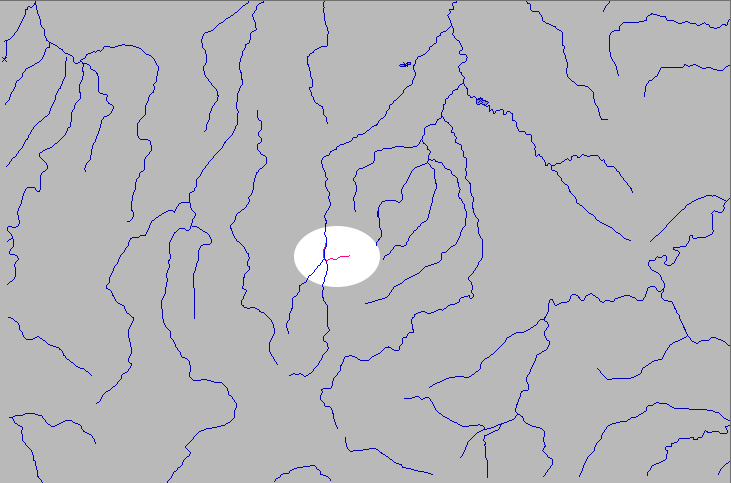
\includegraphics[scale=0.35]{grass014.png}
   %caption of the figure
   \caption{}
   %label of the figure, which has to correspond to \ref{}:
   \label{fig:grass014}
\end{figure}

Quelle est la localisation (Est,Nord) du chemin hydrologique g\'en\'er\'ee rejoignant la rivi\`ere cartographi\'ee, et donc lieu propos\'e pour installer une station de suivit?

\section{Analyse d'habitat}
\subsection{Introduction}

Dans cette session, les \'el\'ements dont vous aurez besoins sont essentiellement (regardez dans la partie RASTER de l'interface principale): 
Le module BUFFERING (r.buffer) Fig.~\ref{fig:grass015}
Le module MAP CALCULATOR (r.mapcalc) Fig.~\ref{fig:grass016}

%\setkeys{Gin}{width=1\textwidth}
\begin{figure}[htbp]
   \centering
   %name of your graphic, without the path AND in PNG (screnshots etc)/PDF (drawings) format:
   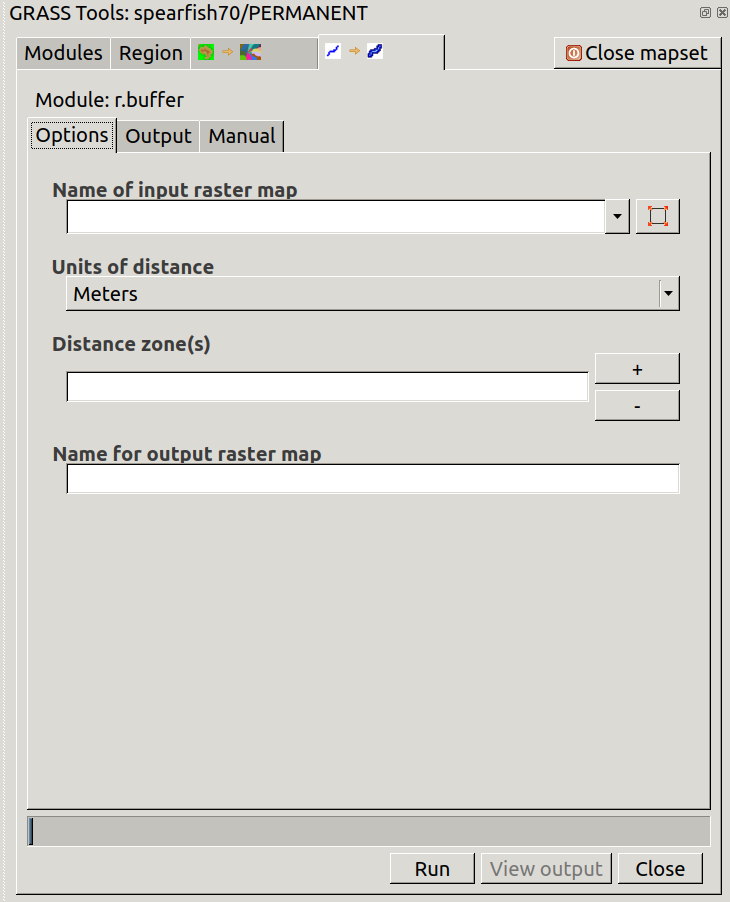
\includegraphics[scale=0.2]{grass015.png}
   %caption of the figure
   \caption{BUFFERING}
   %label of the figure, which has to correspond to \ref{}:
   \label{fig:grass015}
\end{figure}

%\setkeys{Gin}{width=1\textwidth}
\begin{figure}[htbp]
   \centering
   %name of your graphic, without the path AND in PNG (screnshots etc)/PDF (drawings) format:
   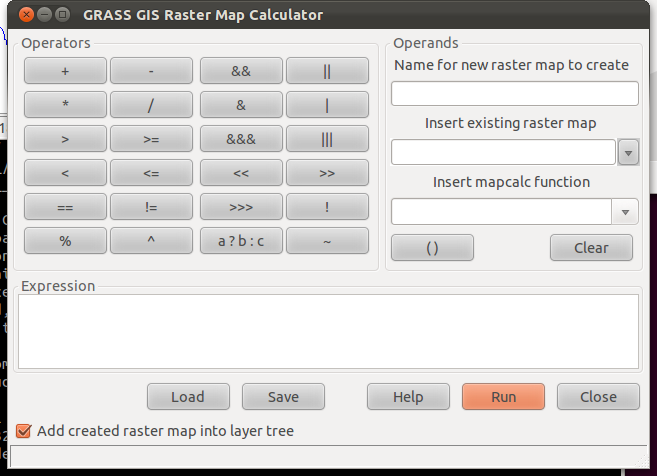
\includegraphics[scale=0.2]{grass016.png}
   %caption of the figure
   \caption{MAP CALCULATOR}
   %label of the figure, which has to correspond to \ref{}:
   \label{fig:grass016}
\end{figure}

\subsection{MISSION DE PRESERVATION D'UN HABITAT}
La Sturnella idemia a r\'ecemment \'et\'e ajout\'ee sur la liste des esp\`eces en danger, et le service en charge de la faune sauvage est en train d'identifier des habitats probables dans la zone sp\'eciale de Spearfish pour prot\'eger contre le d\'eveloppement. Ils ont construit le syst\`emes de points suivant pour cet habitat bas\'e sur les statistiques de pr\'ef\'erences des esp\`eces observ\'ees:

\subsection{SYSTEME DE POINTS POUR L'HABITAT (venant du service de la faune sauvage) }

Num\'ero de carte suivie des conditions environnementales recherch\'ees et enfin les points a donner.
\begin{enumerate}
\item dans 500 m\`etres d'un cours d'eau o\`u la pente <= 5 degr\'es (+2 points)
\item dans 500 m\`etres d'un cours d'eau o\`u la pente >5 degr\'es (+5 points)
\item dans 500 m\`etres d'une route (-5 points)
\item for\^et de conif\`eres (+4 points)
\item for\^et mixte (+1 point)
\item exposition au Nord (aspect de NO \`a NE) (+3 points)
\item exposition \`a l'Ouest ou l'Est (SO au NO ou SE to NE) (+1 point)
\item 1200-1400 m\`etres d'altitude (+2 points)
\item 1400-1600 m\`etres d'altitude (+4 points)
\item over 1600 m\`etres d'altitude (+2 points)
\end{enumerate}

Utilisez r.buffer et r.mapcalc (Map calculator) pour cr\'eer une carte de score d'habitat pour toute la zone, en additionnant tous les scores partiels comme d\'efinis ci-dessus. (conseil: vous devez convertir toutes les valuers nulles des cartes de r\'esultats de buffer en valuers z\'ero)
Quand vous serez termin\'e avec les cartes 1 \`a 10 ci-dessus, additionnez-les toutes en une seule carte que vous pourriez appeler "scoreindivsum". Ensuite, identifiez une zone d'habitat souhaitable en convertissant les valeurs z\'ero des pixels pour tout r\'esultat inf\'erieur \`a 9, et tout pixel dans les 100 m\`etres d'une route (conseil: vous devz faire une nouvelle carte de buffer ici, et enlever ses valeurs nulles pour les calculs). Faites une carte finale que vous pourriez appeler "scorefinal" et changez en les valeurs z\'ero en NULL (..=>Manage null values) pour atteindre la prochaine partie de cet exercice.

\subsection{PREPARATION DES CARTES DE SCORE}

Pour calculer les cartes 1 et 2, utilisez le "Map Calculator" avec un syntaxte comprenant une structure conditionnelle (if). Cel\`a se trouve \^etre dans l'exemple suivant:
\begin{smallverbatim}
if(condition, action_si_vrai, action_si_faux)
\end{smallverbatim}
Dans le cas d'une carte:
\begin{smallverbatim}
if(CarteA==valeur1, score_valeur1, score_valeur2)
\end{smallverbatim}
Dans le cas ou deux cartes sont utilis\'ees ensemble, un syst\`eme conditionnel double peut \^etre d\'ecrit comme ceci:\\

\noindent Un exemple pratique pour la carte num\'ero 1:
\begin{smallverbatim}
if(stream_buff_500==2,if(slope=5,2,0),0)
\end{smallverbatim}
\smallskip
\noindent Vous pouvez ouvrir le GRASS SHELL dans GRASS Tools et entrer cet exemple directement.
\begin{smallverbatim}
r.mapcalc expression="carte1=if(stream_buff_500==2
          ,if(slope=5,2,0),0)"
\end{smallverbatim}

\noindent Dans le cas o\'u l'on voudrait s\'electionner une gamme de valeurs (inclusive ou exclusive), utilisez les op\'erants "OR" et "AND". Questionnez la carte d'aspect (..=>Query with mouse), Est=1 et Nord=+90 degr\'es.\\

\noindent Exemples practiques pour 7a et 7b:
\begin{smallverbatim}
7a) r.mapcalc expression="carte7a=if(aspect<225 
          && aspect>135, 1, 0)"

7b) r.mapcalc expression="carte7b=if(aspect<45 ||
          aspect>314 && aspect!=0, 1, 0)"
\end{smallverbatim}
L'exemple 7b a une contrainte additionnelle ''\&\& aspect !=0'' car la valeur d'aspect 0 veut dire pas d'aspect calcul\'e (g\'en\'eralement en dehors de la zone de donn\'ees de l'image).

\noindent Ce jeu d'instructions montre comment le SIG GRASS produit une reclassification en mode "script". Ceci devient tr\`es utile quand vous avez besoin de r\'e-utiliser une analyse SIG compl\`exe plusieurs fois de suite sur d'autre jeux de donn\'ees par exemple. Pour ce`a il vous suffit simplement d'enregistrer les lignes de commandes dans un fichier texte.

\subsection{HABITAT SCORING SCRIPT}

Num\'ero de carte Conditions environnementales Score \`a donner:

\noindent \textbf{
1) Dans 500 m\`etres des cours d'eau o\`u la pente <= 5 degr\'es: +2 points}
\begin{smallverbatim}
r.buffer input=streams output=bstreams500
 distances=500 units=meters --overwrite

r.null map=bstreams500 null=0

r.mapcalc expression="rbstreams500=
if(_bstreams500==2,1,0)"

r.null map=rbstreams500 null=0
\end{smallverbatim}

\noindent \textbf{
2) Dans 500 m\`etres des cours d'eau o\`u la pente >5 degr\'es: +5 points}
\begin{smallverbatim}
r.buffer input=roads output=broads500 
distances=500 units=meters --overwrite

r.mapcalc expression="s_sl=
if(rbstreams500==1,if(slope<=5,2,5),0)"
\end{smallverbatim}

\noindent \textbf{
3) Dans 500 m\`etres d'une route: -5 points}
\begin{smallverbatim}
r.mapcalc expression="rbroads500=
float(if(_broads500==2,-5.0,0))"
\end{smallverbatim}

\noindent \textbf{
4) for\^et de conif\`eres: +4 points}
\begin{smallverbatim}
r.mapcalc expression="for=
if(vegcover==3,4,0)"
\end{smallverbatim}

\noindent \textbf{
5) for\^et mixte: +1 point}
\begin{smallverbatim}
r.mapcalc expression="for1=
if(vegcover==5,1,0)"
\end{smallverbatim}

\noindent \textbf{
6) Exposition Nord (aspect de NO \`a NE): +3 points}
\begin{smallverbatim}
r.mapcalc expression="exp3=
"if(aspect<=135.0 && aspect>=45.0
 && aspect != 0,3,0)"
\end{smallverbatim}

\noindent \textbf{
7a) Exposition Ouest ou Est (SO \`a NO ou SE \`a NE): +1 point}
\begin{smallverbatim}
r.mapcalc expression="exp1=
if(aspect<45.0 || aspect>314.0,1,0)"

r.mapcalc expression="exp2=
"if(aspect<225.0 && aspect>135.0,1,0)"
\end{smallverbatim}

\noindent \textbf{
7b) 1200-1400 m\`etres d'altitude: +2 points}
\begin{smallverbatim}
r.mapcalc expression="elev1=
if(elevation.10m<1400 && elevation.10m>1200,2,0)"
\end{smallverbatim}

\noindent \textbf{
8) 1400-1600 m\`etres d'altitude: +4 points}
\begin{smallverbatim}
r.mapcalc expression="elev2=
if(elevation.10m<1600 && elevation.10m>=1400,4,0)"
\end{smallverbatim}

\noindent \textbf{
9) plus de 1600 m\`etres d'altitude: +2 points}
\begin{smallverbatim}
r.mapcalc expression="elev3=
if(elevation.10m>=1600,2,0)"
\end{smallverbatim}

\subsection{FINALISATION DE LA CARTE DE SCORE}

\begin{smallverbatim}
r.buffer input=roads output=br100
 distances=100 units=meters --overwrite

r.null map=br100 null=0

r.mapcalc expression="add=
float(s_sl+rbroads500+for+
 for1+exp1+exp2+exp3+elev1+elev2+elev3)"

r.mapcalc expression="clas=if(add>9,1,null())"

r.mapcalc expression="class=
if(clas==1&&br100==0,1,null())"
\end{smallverbatim}

%\setkeys{Gin}{width=1\textwidth}
\begin{figure}[htbp]
   \centering
   %name of your graphic, without the path AND in PNG (screnshots etc)/PDF (drawings) format:
   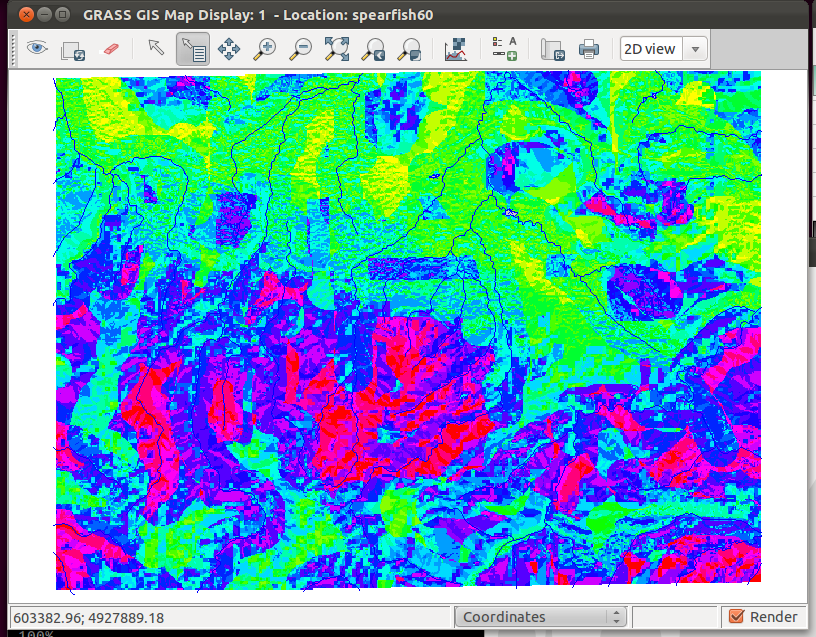
\includegraphics[scale=0.35]{grass021.png}
   %caption of the figure
   \caption{Carte de score}
   %label of the figure, which has to correspond to \ref{}:
   \label{fig:grass021}
\end{figure}

\subsection{METTRE EN BLOC LES ZONES SOUHAITABLES}

Qu'est-ce que ''mettre en bloc''?
Re-cat\'egoriser les donn\'ees dans une carte raster en groupant les pixels qui forment des surfaces continues physiquement en d'uniques cat\'egories.

Maintenant, trouvez les zones discr\`etes/continues (ou clumps) des scores d'aggr\'egation d'habitat. 
Lancez \textit{r.clump (Cherchez: Clump Small Areas) }sur la carte ''\textit{score\_final}'' pour donner \`a chaque bloc son propre num\'ero de cat\'egorie. Vous pourriez appeler la carte r\'esultante ''\textit{score\_clumped}''.

\begin{smallverbatim}
r.clump input=score_final output=score_clumped 
\end{smallverbatim}

Affichez votre nouvelle carte de blocs ''\textit{score\_clumped}''. Elle devrait plus ou moins ressembler \`a cel\`a:Fig.~\ref{fig:grass022}

%\setkeys{Gin}{width=1\textwidth}
\begin{figure}[htbp]
   \centering
   %name of your graphic, without the path AND in PNG (screnshots etc)/PDF (drawings) format:
   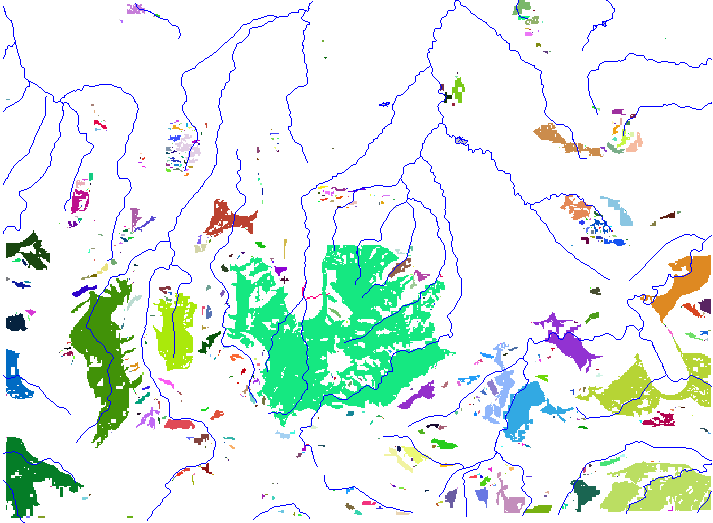
\includegraphics[scale=0.35]{grass022.png}
   %caption of the figure
   \caption{Carte des blocs}
   %label of the figure, which has to correspond to \ref{}:
   \label{fig:grass022}
\end{figure}


Puisque cette esp\`ece est mieux dans de larges blocs, faites une extraction des blocs sup\'erieurs a 50 hectares dans une carte sp\'epar\'ee. Vous pourriez utilisez le terminal pour reclassifier par seuil de surface sup\'erieur \`a 50 hectares:

\begin{smallverbatim}
r.reclass.area input = score_final greater=50 
 output=selected_habitat_area
\end{smallverbatim}

R\'esultat ''selected\_habitat\_area'' \`a ce niveau devrait \^etre similaire \`a ceci:Fig.~\ref{fig:grass023}

%\setkeys{Gin}{width=1\textwidth}
\begin{figure}[htbp]
   \centering
   %name of your graphic, without the path AND in PNG (screnshots etc)/PDF (drawings) format:
   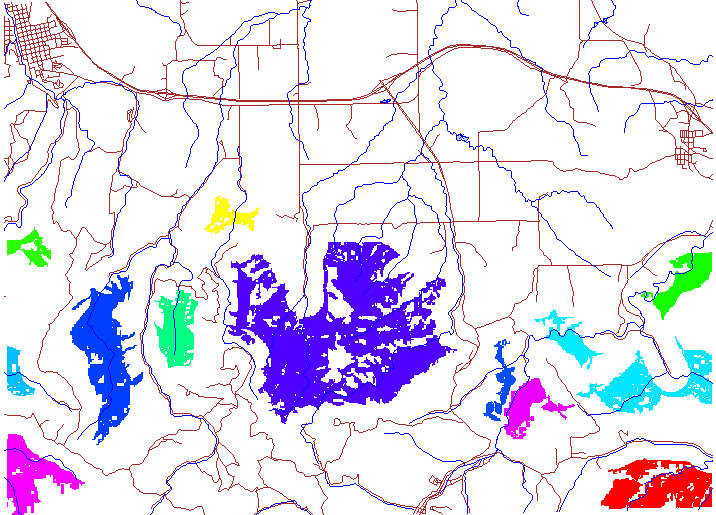
\includegraphics[scale=0.35]{grass023.png}
   %caption of the figure
   \caption{Zones d'habitat s\'electionn\'ees}
   %label of the figure, which has to correspond to \ref{}:
   \label{fig:grass023}
\end{figure}

\subsection{EXPORT DES RESULTATS SOUS FORMAT VECTORIEL}
Puisque nos clients travaillent sous SIG \`a format vectoriel, nous allons convertir les r\'esultats en format vectoriel et les exporter de GRASS \`a ESRI shapefile.

Vectorisez la carte de blocs que vous venez de produire (Recherchez ''conversion'' dans GRASS Tools) et v\'erifiez que vous avez effectivement cr\'ee une carte vectorielle \`a \'el\'ements de type polygones en affichant votre couche vectorielle. Fig.~\ref{fig:grass024}

%\setkeys{Gin}{width=1\textwidth}
\begin{figure}[htbp]
   \centering
   %name of your graphic, without the path AND in PNG (screnshots etc)/PDF (drawings) format:
   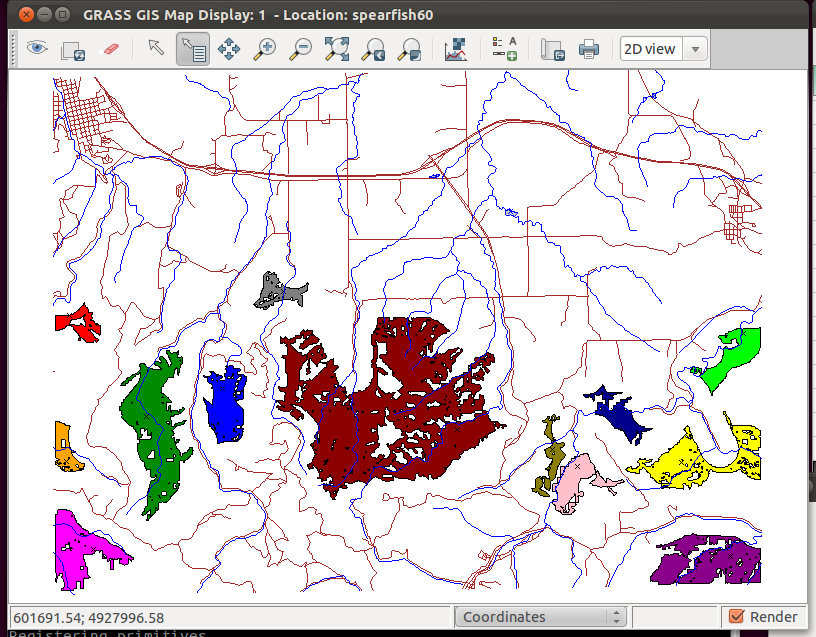
\includegraphics[scale=0.35]{grass024.png}
   %caption of the figure
   \caption{Export de fichier vectoriel}
   %label of the figure, which has to correspond to \ref{}:
   \label{fig:grass024}
\end{figure}

Exportez ce fichier vectoriel d'habitat avec ''\textit{roads}'' et ''\textit{streams}'' aussi en format shapefile. Soyez s\^ur que vous exportez le m\^eme type d'\'el\'ements vectoriels (area pour ''\textit{selected\_habitat\_area}'' et lines pour ''\textit{roads}'' et ''\textit{streams}''). Affichez et questionnez ces fichiers dans le SIG Quantum.

\begin{smallverbatim}
v.out.ogr input=selected_habitat_area type=area
 dsn=QGISDATA layer=1 format=ESRI_Shapefile

v.out.ogr input=roads type=line dsn=QGISDATA
 layer=1 format=ESRI_Shapefile

v.out.ogr input=streams type=line dsn=QGISDATA
 layer=1 format=ESRI_Shapefile
\end{smallverbatim}

\noindent \textbf{Pour les t\'em\'eraires ...}

Cette esp\`ece est assez intol\'erante des perturbations aux fronti\`eres de zones, donc vous devriez faire un poids plus lourd pour les zones internes que frontali\`eres des blocs d'habitat. \\
Cr\'eez des buffers internes concentriques de 100 m\`etres pour chaque bloc, avec un poids de 
\begin{enumerate}
\item pour le premier buffer en fronti\`ere (0-100 m\`etres internes), 
\item pour le second vers l'interieur (100-200 m\`etres), 3 pour 200-300 m\`etres, etc..., 
\item quand aux pixels en dehors des blocs, leurs valeurs sont de z\'ero.
\end{enumerate}

\noindent Pour cel\`a:

\begin{enumerate}
\item Utilisez \textit{r.mapcalc} pour multiplier la carte d'habitat par les poids des buffers internes.
\item Maintenant lancez \textit{r.volume }sur cette carte r\'esultante pour obtenir la somme et la moyenne de chaque bloc.
\item Utilisez  \textit{awk} pour cr\'eer des fichiers de r\`egles de r\'eclassification, puis utilisez \textit{r.reclass} pour cartographier les blocs par somme et moyenne.
\item Quel bloc a le nouveau total maximum? Lequel a la nouvelle moyenne maximum?
\item Utilisez \textit{r.grow} pour cr\'eer une carte de fronti\`eres de blocs (soustraire les cartes d'origines aux cartes r\'esultantes).
\item Utilisez les cartes de fronti\`eres de blocs pour indexer le p\'erimetre de chaque bloc majeur. 
\item Calculez la compacit\'e (surface divis\'ee par le carr\'e du p\'erimetre) de chaque bloc. 
\item Cartographiez les blocs par compacit\'e. 
\item Cr\'eez un script d'affichage cool pour d\'emontrer vos proc\'edures et expliquez ce que vous avez trouv\'e.
\end{enumerate}

\subsection{Exemple de script}

\noindent Veuillez mettre ceci dans un fichier \textit{script.sh} \textup{et dans un } \textit{Terminal} \textup{ \'ecrivez: ''chmod 0755} \textit{script.sh''}\textup{. Ensuite vous pouvez lancer le script } en \'ecrivant la commande: ''./script.sh'' (Linux/Mac). \\
\noindent Ce script utilise une veille version de r.mapcalc, convertissez les lignes de commande en utilisant la forme \textit{r.mapcalc expression=''carte=carte1+carte2''}. \\
\noindent Ce script contient des commandes d'affichage automatique des nouvelles cartes, ces commandes (d.mon, d.rast, d.vect) ne fonctionneront pas dans l'interface de QGIS car elles sont natives seulement de GRASS GIS. 

\begin{smallverbatim}
#!/bin/bash
# Noms des variables de cartes
dem=elevation.dem
r=roads
s=streams
#Set resolution and extents from elevation.10m
d.region raster=$dem
# buffer cours d'eau et routes
_bs=bstreams500
_br=broads500
# reclassement des buffer cours d'eau et routes
_rbs=rbstreams500
_rbr=rbroads500
#--------------------------------------------------
# Presentation generale: Debut Affichage 0
#--------------------------------------------------
d.mon start=wx0
d.erase color=grey
d.rast map=$dem
sleep 1
d.vect map=$r color=brown
sleep 1
d.vect map=$s color=blue
sleep 1
d.barscale bcolor=white tcolor=black at=30.0,95.0
sleep 2
#--------------------------------------------------
# Creation de buffer: Debut Affichage 1
#--------------------------------------------------
d.mon start=wx1
d.mon select=wx1
d.erase color=grey
r.buffer input=$s output=$_bs distances=500
 units=meters --overwrite
r.null map=$_bs null=0
d.rast map=$_bs
d.vect map=$s color=blue
d.barscale bcolor=white tcolor=black at=30.0,95.0
r.buffer input=$r output=$_br distances=500
 units=meters --overwrite
r.null map=$_br null=0
d.rast map=$_br
d.vect map=$s color=blue
d.barscale bcolor=white tcolor=black at=30.0,95.0
#--------------------------------------------------
# Reclassification: Debut Affichage 2
#--------------------------------------------------
d.mon start=wx2
d.mon select=wx2
d.erase color=grey
echo "...Reclassification..."
r.mapcalc expression="$_rbs=if($_bs==2,1,0)"
r.mapcalc expression="s_sl=if($_rbs==1,if(slope<=5,2,5),0)"
r.mapcalc expression="$_rbr=float(if($_br==2,-5.0,0))"
r.mapcalc expression="for=if(vegcover==3,4,0)"
r.mapcalc expression="for1=if(vegcover==5,1,0)"
r.mapcalc expression="exp1=if(aspect<45.0 || aspect>314.0 &&
 aspect != 0.0,1,0)"
r.mapcalc expression="exp2=if(aspect<225.0 && aspect>135.
 0,1,0)"
r.mapcalc expression="exp3=if(aspect<=135.0 && aspect>=45.0,
 3,0)"
r.mapcalc expression="elev1=if($dem<1400 && $dem>1200,2,0)"
r.mapcalc expression="elev2=if($dem<1600 && $dem>=1400,4,0)"
r.mapcalc expression="elev3=if($dem>=1600,2,0)"
#--------------------------------------------------
r.buffer input=$r output=br100 distances=100
 units=meters --overwrite
r.null map=br100 null=0
r.mapcalc expression="add=float(s_sl+$_rbr+for+for1+
 exp1+exp2+exp3+elev1+elev2+elev3)"
r.mapcalc expression="clas=if(add{>9,1,null())"
r.mapcalc expression="class=if(clas==1&&br100==0,1,null())"
echo "Reclassification...Fin."
d.rast map="$_rbs"
sleep 1
d.rast map="s_sl"
d.rast map="$_rbr"
d.rast map="for"
d.rast map="for1"
d.rast map="exp1"
d.rast map="exp2"
d.rast map="exp3"
d.rast map="elev1"
d.rast map="elev2"
d.rast map="elev3"
d.rast map="br100"
sleep 1
#r.colors color=grey map="add"
d.rast map="add"
sleep 1
d.rast map="class"
sleep 1
#d.erase
d.vect map="$s" color=blue
d.vect map="$r" color=brown
d.barscale bcolor=white tcolor=black at=30.0,95.0
sleep 5
g.remove
rast="$_rbs,s_sl,$_rbr,for,for1"}
g.remove
rast="exp1,exp2,exp3,elev1"}
g.remove
rast="elev2,elev3,br100,add"}
g.remove rast="$_bs,$_br,clas"}
sleep 1
echo ""
echo "fin"
sleep 1
#--------------------------------------------------
# Mettre en bloc: Debut Affichage 3
#--------------------------------------------------
d.mon start=wx3
d.mon select=wx3
d.erase color=grey
g.remove rast=clump.clump._rclumpnew
r.clump input=class output=clump --overwrite
r.colors color=gyr map="clump"
d.rast map="clump"
sleep 1
r.reclass.area input=clump greater=50
 output=rclumpnew --overwrite
r.colors color=gyr map="rclumpnew"
d.erase color=white
d.rast map="rclumpnew"
sleep 1
d.vect map="streams" color=blue
d.vect map="roads" color=brown
d.barscale bcolor=white tcolor=black at=30.0,95.0
sleep 1
g.remove rast="clump,class"
#--------------------------------------------------
# R2V et Export: Debut Affichage 4
#--------------------------------------------------
d.mon start=wx4
d.mon select=wx4
d.erase color=white
r.to.vect -s input=rclumpnew output=rclump
 feature=area --overwrite
d.vect -c map=rclump type=area color=black
d.vect map="streams" color=blue
d.vect map="roads" color=brown
d.barscale bcolor=white tcolor=black at=30.0,95.0
sleep 1
v.out.ogr input=rclump type=area dsn=QGISDATA
 layer=1 format=ESRI_Shapefile --overwrite
g.remove rast="rclumpnew"
g.remove vect="rclump"
d.mon stop=wx4
d.mon stop=wx3
d.mon stop=wx2
d.mon stop=wx1
d.mon stop=wx0
\end{smallverbatim}

%\address{Yann Chemin\\
%  \url{http://grass.osgeo.org}\\
 % \email{yann.chemin@gmail.com}}

%%% Local Variables: 
%%% mode: latex
%%% TeX-master: main_document.tex
%%% End: 

